\documentclass[a4paper]{jlreq}

% Build-log noise reduction for this teaching material.
\usepackage{../sty/latex-intro-warning-filter}

% Japanese text setup for LuaLaTeX. Keep this near the top.
\usepackage[haranoaji]{luatexja-preset}

% Page layout. Reports are easier to read when margins are explicit.
\usepackage[margin=25truemm,headheight=18pt]{geometry}

% Math basics. amsmath/mathtools are the core pair for report writing.
\usepackage{amsmath}
\usepackage{amssymb}
\usepackage{mathtools}
\usepackage{bm}

% Figures and tables.
\usepackage{float}
\usepackage{graphicx}
\usepackage{booktabs}

% Code examples and gentle highlighting inside the handout.
\usepackage{datetime2}
\usepackage{fancyhdr}
\usepackage{fancyvrb}
\usepackage{lastpage}
\usepackage{xcolor}

% Bibliography and hyperlinks. hyperref stays near the end.
\usepackage[backend=biber,style=numeric,sorting=nyt]{biblatex}
\usepackage[colorlinks=true,linkcolor=blue!50!black,citecolor=blue!50!black,urlcolor=blue!70!black]{hyperref}

\addbibresource{../bib/references.bib}
\numberwithin{equation}{section}
\DTMsetdatestyle{iso}
\setlength{\headheight}{18pt}

\pagestyle{fancy}
\fancyhf{}
\fancyhead[L]{\DTMtoday}
\fancyhead[R]{\thepage/\pageref{LastPage}}
\renewcommand{\headrulewidth}{0.4pt}

\DefineVerbatimEnvironment{codeblock}{Verbatim}{
  fontsize=\small,
  frame=single,
  xleftmargin=1.5em,
  xrightmargin=1.5em
}

\newcommand{\pkg}[1]{\textsf{#1}}
\newcommand{\cmd}[1]{\texttt{\textbackslash#1}}
\newcommand{\env}[1]{\texttt{#1}}
\newcommand{\file}[1]{\texttt{#1}}
\newcommand{\materialtitle}{LuaLaTeX + jlreq ではじめる日本語\LaTeX{}入門}

\fancyhead[C]{\nouppercase{\materialtitle}}

\title{\materialtitle}
\author{kska6}
\date{\today}

\begin{document}
\maketitle
\tableofcontents
\newpage

\section{この資料の目的}

この資料は、LuaLaTeX と \texttt{jlreq} を前提に、日本語のレポートや論文を書き始めるための入門資料です。
目標は、次の 3 点です。

\begin{itemize}
  \item まずコンパイルが通る最小構成を作れるようになる
  \item 数式、図表、参考文献、相互参照を段階的に追加できるようになる
  \item 卒業論文や技術文書へ拡張しやすい書き方を身につける
\end{itemize}

この資料では「何を書くとどうなるか」だけでなく、「なぜその環境や記法を使うのか」も重視します。
\LaTeX{}では見た目を直接いじるより、文書の構造を明示して書く方が、長い文書になったときに強くなります。

\section{まず動かす}

\subsection{最小構成}

最初の目標は、機能を盛り込むことではなく、コンパイルを成功させることです。
このリポジトリには、最小構成の例として \file{src/minimal.tex} を用意しています。

\begin{codeblock}
\documentclass{jlreq}

\title{LaTeXの最小構成}
\author{氏名}
\date{\today}

\begin{document}
\maketitle

\section{はじめに}

これはLuaLaTeXで作成する最小構成の文書です。

\section{数式の例}

文中の数式は $E = mc^2$ のように書きます。

\begin{equation}
F = ma
\end{equation}

\end{document}
\end{codeblock}

この段階では、\cmd{documentclass}、\cmd{begin\{document\}} と \cmd{end\{document\}}、\cmd{section}、\env{equation} だけ追えれば十分です。
最初から多くの package を入れるより、最小構成が通る状態を基準にした方が、問題が起きたときに切り分けやすくなります。

\subsection{コンパイル}

最小構成は、次のようにコンパイルできます。

\begin{codeblock}
latexmk -lualatex src/minimal.tex
\end{codeblock}

\texttt{lualatex} は実際に PDF を作るエンジンで、\texttt{latexmk} は必要な回数だけ再実行したり、参考文献ツールを呼び出したりする管理役です。
普段の作業では、\texttt{lualatex} を直接何度も叩くより、\texttt{latexmk} を入口にそろえる方が運用しやすくなります。

\subsection{\file{hello.tex} でエンジンを見る}

\file{minimal.tex} の次は、\file{src/hello.tex} を使って「いま何のエンジンで動いているか」を確認すると理解しやすくなります。
\file{hello.tex} は文書の内容を増やすための例ではなく、コンパイル系統の違いを見るための小さなサンプルです。

\begin{codeblock}
latexmk -lualatex src/hello.tex
\end{codeblock}

このファイルをビルドすると、出力には \texttt{Hello, LuaLaTeX!} のように、実際に使われたエンジン名が現れます。
つまり、\file{minimal.tex} で「まず通す」、\file{hello.tex} で「何で通しているかを確認する」という二段構えにすると、入門時の導線が整理しやすくなります。

\section{LuaLaTeX と jlreq}

\subsection{なぜ LuaLaTeX を使うのか}

日本語文書では、エンジンと日本語処理の相性が重要です。
LuaLaTeX は \pkg{luatexja} 系と組み合わせやすく、日本語を比較的素直に扱えます。
入門段階では、「日本語レポートを通しやすい構成」として LuaLaTeX を選ぶ、と理解すれば十分です。

ここで \file{hello.tex} を見ると、「エンジン」とは \file{.tex} を処理して PDF へつなぐ実体であり、\texttt{LuaLaTeX} や \texttt{XeLaTeX} などの違いがあることを、抽象論だけでなく出力結果として確認できます。

\subsection{なぜ jlreq を使うのか}

\texttt{jlreq} は日本語組版を意識して設計された文書クラスです。
英語向けの標準クラスを無理に流用するより、日本語の見出しや版面を自然に扱いやすくなります。
レポート用途では既定の \texttt{article} 相当で始めれば十分で、長い文書では次のように切り替えます。

\begin{codeblock}
\documentclass[a4paper,report]{jlreq}
\documentclass[a4paper,book]{jlreq}
\end{codeblock}

\texttt{report} は章立てのある報告書向け、\texttt{book} はさらに長い冊子向けです。
講義レポートなら既定設定、卒論や章構成を持つ文書なら \texttt{report} をまず検討すると整理しやすくなります。

\section{プリアンプルと package}

\subsection{プリアンプルとは何か}

\cmd{begin\{document\}} より前に書く設定部分をプリアンプルと呼びます。
ここには、文書全体で使う package、ページ設定、番号付け、独自コマンドなどを書きます。
本文の途中で毎回同じ設定を書くのではなく、共通設定を一箇所にまとめるための領域だと考えるとよいです。

\subsection{この資料で使う package}

この資料の冒頭では、次のように package を読み込んでいます。

\begin{codeblock}
% Japanese text setup for LuaLaTeX. Keep this near the top.
\usepackage[haranoaji]{luatexja-preset}

% Page layout. Reports are easier to read when margins are explicit.
\usepackage[margin=25truemm]{geometry}

% Math basics. amsmath/mathtools are the core pair for report writing.
\usepackage{amsmath}
\usepackage{amssymb}
\usepackage{mathtools}
\usepackage{bm}

% Figures and tables. float is for the optional [H] placement.
\usepackage{graphicx}
\usepackage{booktabs}

% Bibliography and hyperlinks. hyperref stays near the end.
\usepackage[backend=biber,style=numeric,sorting=nyt]{biblatex}
\usepackage{hyperref}
\end{codeblock}

読み込み順にも理由があります。
\pkg{luatexja-preset} は日本語環境の基盤なので早めに置き、\pkg{hyperref} は他の機能にリンクを付ける都合で後ろ側に置くのが定石です。
\pkg{mathtools} は \pkg{amsmath} を拡張する package なので、\pkg{amsmath} の後に読みます。

\subsection{不要な package を増やさない}

package は便利ですが、増やしすぎると依存関係や競合が見えにくくなります。
特に入門段階では、次の順で考えると安全です。

\begin{enumerate}
  \item まず最小構成で通す
  \item 必要な機能が出たときに package を 1 つずつ追加する
  \item 追加理由をコメントで残す
\end{enumerate}

たとえば、図を入れない文書に \pkg{graphicx} は不要です。
参考文献をまだ扱わない段階で \pkg{biblatex} を入れなくても構いません。
「今この文書に何の機能が必要か」を基準にすると、保守しやすいプリアンプルになります。

\section{文章の構造を書く}

\subsection{見出し}

\LaTeX{}では、見た目を大きくするより、見出しとしての役割を命令で示します。

\begin{codeblock}
\section{実験方法}
\subsection{装置}
\subsection{手順}
\end{codeblock}

この書き方にすると、見出し番号や目次との連携が自動化されます。
後から節を追加しても番号を手で直す必要がありません。

\subsection{段落と改行}

空行は段落の区切り、\verb|\\| は行の折り返しです。
文章を書くときは、見た目をそろえるために \verb|\\| を多用するのではなく、段落構造で整理します。
\verb|\\| は住所や詩のように、意味として改行したい場合に限って使う方が安全です。

\subsection{箇条書き}

箇条書きは、文章を構造化して読みやすくするために使います。
単に行頭へ記号を並べるのではなく、項目のまとまりを環境として表します。

\subsubsection{\env{itemize}}

\env{itemize} は順序を持たない列挙です。

\begin{codeblock}
\begin{itemize}
  \item 目的を書く
  \item 方法を書く
  \item 結果を書く
\end{itemize}
\end{codeblock}

項目ごとに \cmd{item} を書くと、字下げや記号の配置が自動で整います。

\subsubsection{\env{enumerate}}

\env{enumerate} は順序を持つ列挙です。
手順や実験プロセスの説明でよく使います。

\begin{codeblock}
\begin{enumerate}
  \item データを整理する
  \item グラフを作成する
  \item 考察を書く
\end{enumerate}
\end{codeblock}

\subsubsection{ネスト}

箇条書きは入れ子にできます。
ただし深くしすぎると読みにくくなるため、二段程度までに抑える方が実用的です。

\begin{codeblock}
\begin{itemize}
  \item レポート本文
  \begin{enumerate}
    \item はじめに
    \item 実験方法
    \item 結果と考察
  \end{enumerate}
  \item 参考文献
\end{itemize}
\end{codeblock}

\section{数式を書く}

\subsection{インライン数式}

文中に短い数式を入れるときは、\verb|$...$| を使います。

\begin{codeblock}
質量 $m$ の物体に力 $F$ が加わるとき、加速度は $a = F/m$ です。
\end{codeblock}

本文の流れを切らずに記号を説明したいときに向いています。
逆に、式変形の途中や参照したい式までインラインで詰め込むと読みにくくなります。

\subsection{\env{equation}}

\env{equation} は、独立した 1 本の式を番号付きで示したいときに使います。

\begin{codeblock}
\begin{equation}
E = mc^2
\label{eq:energy}
\end{equation}
\end{codeblock}

本文中から \eqref{eq:sample-newton} のように参照したいなら、\env{equation} を使う価値があります。
独立した式に番号を持たせることで、後から説明や考察で再利用しやすくなるためです。

\begin{equation}
F = ma
\label{eq:sample-newton}
\end{equation}

\subsection{\env{align}}

\env{align} は、複数行の式をそろえて書きたいときに使います。
等号の位置を合わせると、変形の流れが読み取りやすくなります。

\begin{codeblock}
\begin{align}
y &= (x + 1)^2 \\
  &= x^2 + 2x + 1
\end{align}
\end{codeblock}

\begin{align}
y &= (x + 1)^2 \\
  &= x^2 + 2x + 1
\label{eq:expanded}
\end{align}

\env{equation} と \env{align} の違いは、主に「1 行を独立して見せたいか」「複数行の対応関係を見せたいか」です。
1 本の式なら \env{equation}、変形を追わせたいなら \env{align} を使います。

\subsection{\env{aligned}}

\env{aligned} は単独では使わず、通常は \env{equation} などの中に入れて使います。
「式全体としては 1 番号にしたいが、中では複数行をそろえたい」ときに便利です。

\begin{codeblock}
\begin{equation}
\begin{aligned}
f(x)
  &= (x + 1)(x - 1) \\
  &= x^2 - 1
\end{aligned}
\label{eq:aligned-example}
\end{equation}
\end{codeblock}

\begin{equation}
\begin{aligned}
f(x)
  &= (x + 1)(x - 1) \\
  &= x^2 - 1
\end{aligned}
\label{eq:aligned-example}
\end{equation}

\env{align} は各行を並べるための外側の環境、\env{aligned} は他の数式環境の中で行揃えだけをしたいときの内側の環境、と覚えると区別しやすくなります。

\subsection{\env{cases} と \env{dcases}}

場合分けを書くときは \env{cases} を使います。

\begin{codeblock}
\begin{equation}
|x| =
\begin{cases}
  x & (x \geq 0) \\
  -x & (x < 0)
\end{cases}
\end{equation}
\end{codeblock}

\begin{equation}
|x| =
\begin{cases}
  x & (x \geq 0) \\
  -x & (x < 0)
\end{cases}
\label{eq:abs-cases}
\end{equation}

\env{cases} の各行は本文スタイルで組まれるため、分数などが少し小さく見えることがあります。
そこで \pkg{mathtools} の \env{dcases} を使うと、各行が displaystyle で組まれ、式が見やすくなる場合があります。

\begin{codeblock}
\begin{equation}
f(n) =
\begin{dcases}
  \dfrac{n}{2} & (n \text{ が偶数}) \\
  \dfrac{3n + 1}{2} & (n \text{ が奇数})
\end{dcases}
\end{equation}
\end{codeblock}

\begin{equation}
f(n) =
\begin{dcases}
  \dfrac{n}{2} & (n \text{ が偶数}) \\
  \dfrac{3n + 1}{2} & (n \text{ が奇数})
\end{dcases}
\label{eq:dcases-example}
\end{equation}

短い式だけなら \env{cases} で十分ですが、分数や総和のように大きめの記号を含む場合は \env{dcases} の方が読みやすいことがあります。

\subsection{連立方程式}

連立方程式では、左側の大きな波括弧と、各式の揃えを同時に扱いたくなります。
このとき \env{aligned} を使うと、「全体は 1 個の数式」として扱いながら中だけ整列できます。

\begin{codeblock}
\begin{equation}
\begin{cases}
\begin{aligned}
2x + y &= 1 \\
x - y &= 3
\end{aligned}
\end{cases}
\end{equation}
\end{codeblock}

\begin{equation}
\left\{
\begin{aligned}
2x + y &= 1 \\
x - y &= 3
\end{aligned}
\right.
\label{eq:simultaneous}
\end{equation}

連立方程式で \env{aligned} を使う理由は、各行の等号位置をそろえつつ、式全体の番号を 1 つにまとめやすいからです。
独立した複数の式ではなく、1 組の方程式として見せたい場面に向いています。

\subsection{ベクトルと太字}

数式中では、ベクトルや行列を太字で表したいことがあります。
\cmd{boldsymbol} でも書けますが、\pkg{bm} を入れておくと \cmd{bm} で簡潔に書けます。

\begin{codeblock}
\begin{equation}
\bm{F} = m\bm{a}
\end{equation}
\end{codeblock}

\begin{equation}
\bm{F} = m\bm{a}
\label{eq:bold-vector}
\end{equation}

\subsection{数式番号と参照}

数式番号を本文で手打ちしてはいけません。
番号は編集のたびにずれるので、式の直後に \cmd{label} を置き、本文では \cmd{eqref} で参照します。

\begin{codeblock}
\begin{equation}
F = ma
\label{eq:newton}
\end{equation}

式 \eqref{eq:newton} より、力と加速度は比例します。
\end{codeblock}

\cmd{ref} は一般の番号参照、\cmd{eqref} は数式参照で丸括弧まで含めて出したいときに使います。
式番号を「(3.1)」のように直接打つより、修正に強い書き方です。

\section{図表を書く}

\subsection{図}

画像を入れるには \pkg{graphicx} と \cmd{includegraphics} を使います。
図番号を手打ちするのではなく、\cmd{caption} と \cmd{label} を組み合わせて管理します。

\begin{codeblock}
\begin{figure}[tb]
  \centering
  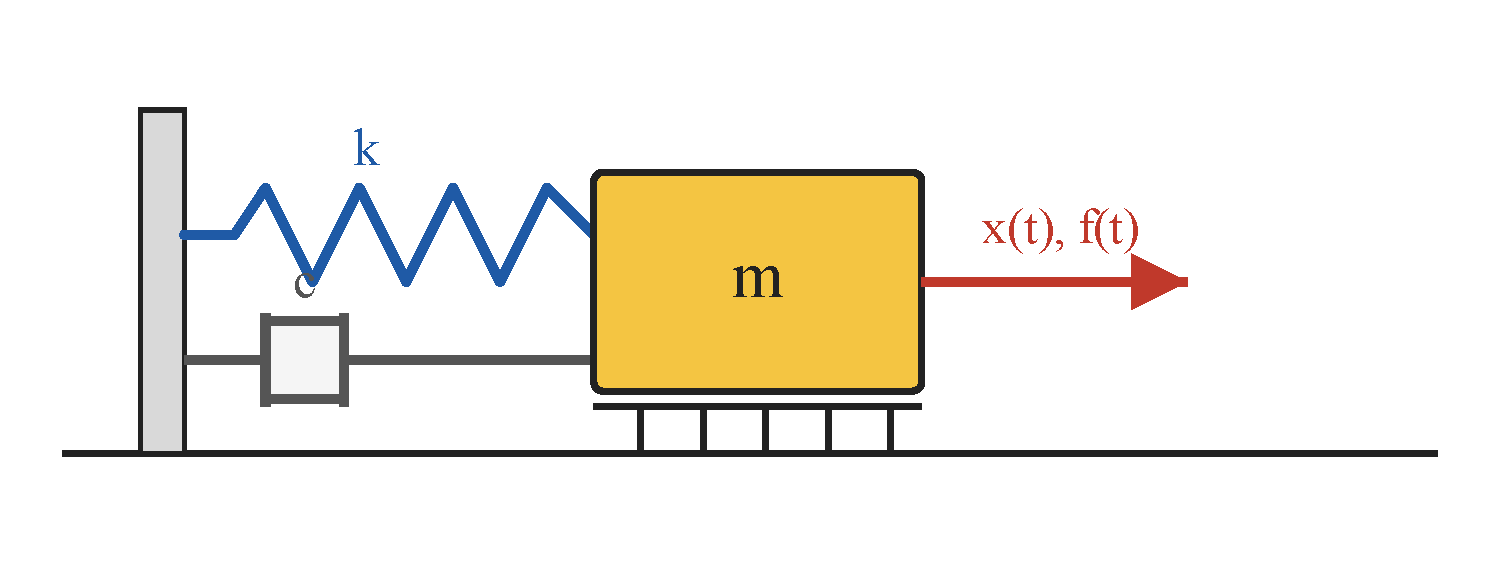
\includegraphics[width=.7\linewidth]{../fig/mass-spring-damper.pdf}
  \caption{質量--ばね--ダンパ系}
  \label{fig:mass-spring-damper}
\end{figure}
\end{codeblock}

\begin{figure}[tb]
  \centering
  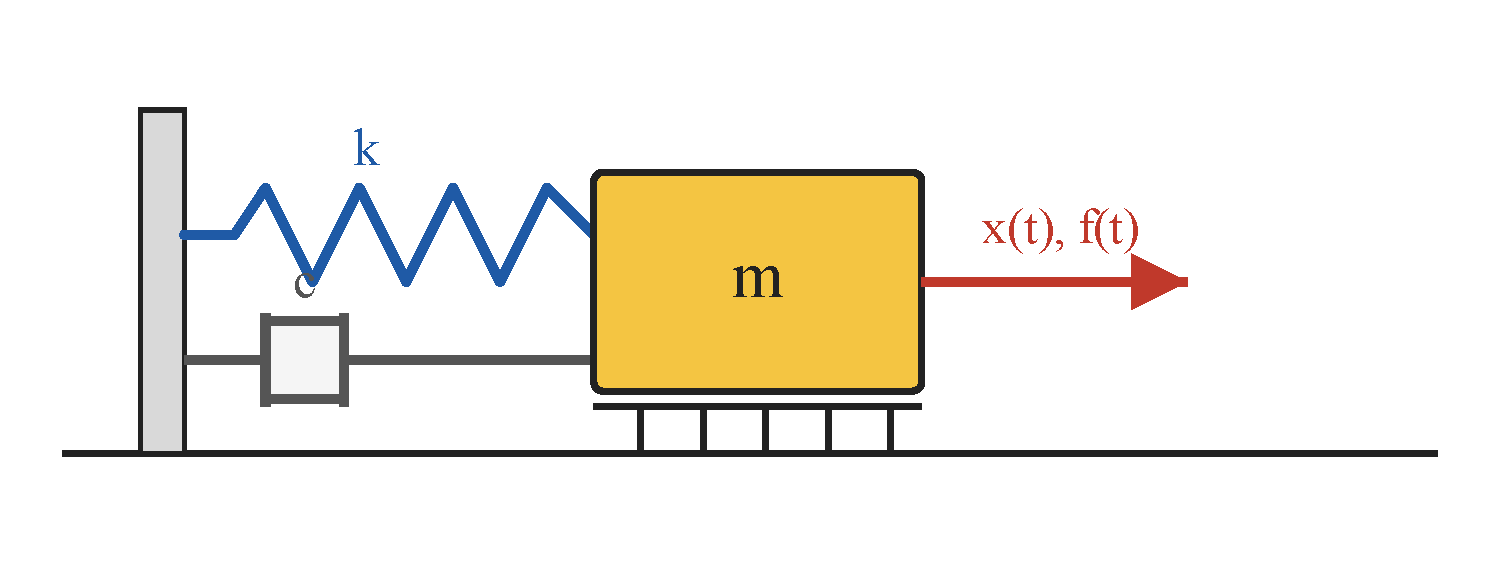
\includegraphics[width=.7\linewidth]{../fig/mass-spring-damper.pdf}
  \caption{質量--ばね--ダンパ系}
  \label{fig:mass-spring-damper}
\end{figure}

\cmd{label} は \cmd{caption} の後に置きます。
図番号は \cmd{caption} が進めるため、その前に \cmd{label} を置くと意図しない番号を拾うことがあります。
また、画像ファイルは \file{fig/} に分けておくと、本文ソースと素材を整理しやすくなります。

\subsection{表}

表では \env{table} が浮動体、\env{tabular} が中身の表組です。
役割が違うので、両方の役目を分けて理解すると混乱しにくくなります。

\begin{codeblock}
\begin{table}[tb]
  \centering
  \caption{モデルのパラメータ}
  \label{tab:parameters}
  \begin{tabular}{lll}
    \toprule
    記号 & 意味 & 単位 \\
    \midrule
    $m$ & 質量 & kg \\
    $k$ & ばね定数 & N/m \\
    $c$ & 減衰係数 & N s/m \\
    \bottomrule
  \end{tabular}
\end{table}
\end{codeblock}

\begin{table}[tb]
  \centering
  \caption{モデルのパラメータ}
  \label{tab:parameters}
  \begin{tabular}{lll}
    \toprule
    記号 & 意味 & 単位 \\
    \midrule
    $m$ & 質量 & kg \\
    $k$ & ばね定数 & N/m \\
    $c$ & 減衰係数 & N s/m \\
    \bottomrule
  \end{tabular}
\end{table}

\pkg{booktabs} を使うと、\cmd{toprule}、\cmd{midrule}、\cmd{bottomrule} で見やすい横罫線を書けます。
実務や論文では、縦罫線を増やすより、余白と横罫線で整理する方が読みやすいことが多くあります。

\subsection{配置指定と \texttt{[H]}}

\env{figure} や \env{table} は浮動体なので、ソースに書いた位置へ必ずそのまま出るとは限りません。
通常は \verb|[tb]| や \verb|[htbp]| のように候補位置を与えて、配置は \LaTeX{} にある程度任せる方が紙面を崩しにくくなります。

どうしても「この位置にそのまま置きたい」ときだけ、\pkg{float} の \verb|[H]| を使います。

\begin{codeblock}
\begin{figure}[H]
  \centering
  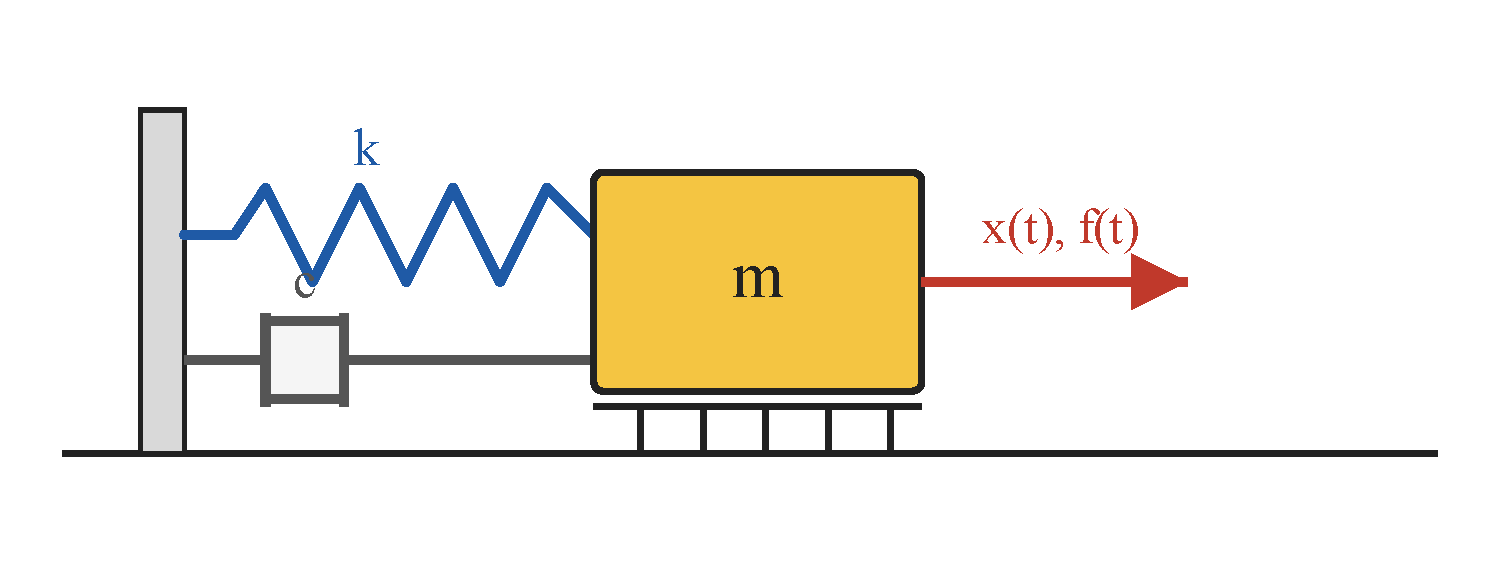
\includegraphics[width=.7\linewidth]{../fig/mass-spring-damper.pdf}
  \caption{この位置に固定したい図}
  \label{fig:fixed-example}
\end{figure}
\end{codeblock}

\verb|[H]| は便利ですが、使いすぎると図表が詰まり、かえって読みづらくなることがあります。
まずは通常の浮動配置で様子を見て、本当に固定が必要な図表だけに絞る方が実運用では安全です。

\subsection{図表参照}

図や表も番号を手打ちせず、\cmd{ref} を使います。
たとえば、図 \ref{fig:mass-spring-damper} や表 \ref{tab:parameters} のように参照できます。
これにより、図表を追加して番号がずれても本文を手で追い直す必要がありません。

\section{ラベルと参照}

\subsection{基本}

\cmd{label} は「この場所に名前を付ける」命令、\cmd{ref} は「その番号を呼び出す」命令です。
相互参照の基本は次の形です。

\begin{codeblock}
\section{結果}
\label{sec:result}

第\ref{sec:result}節で結果を述べる。
\end{codeblock}

式なら \cmd{eqref}、図表や節なら \cmd{ref} を使う、という整理で十分です。
いずれの場合も、番号そのものを本文へ打ち込まないことが重要です。

\subsection{hyperref}

\pkg{hyperref} を入れると、目次、参照、URL が PDF 上でクリック可能になります。
長いレポートや論文では、参照先へ飛べるだけで読みやすさが大きく変わります。
そのため、入門段階でも相互参照を使う文書では導入しておく価値があります。

\subsection{zref}

\pkg{zref} は、相互参照をより柔軟に扱いたいときに使う発展的な package です。
基本的なレポートなら \cmd{label} と \cmd{ref}、\cmd{eqref}、そして \pkg{hyperref} で十分ですが、参照に付ける情報を増やしたいときに \pkg{zref} が候補になります。

たとえば、次のような場面で検討できます。

\begin{itemize}
  \item 図、表、式、節の参照表記をまとめて整えたい
  \item 番号だけでなくページ情報なども扱いたい
  \item 複数種類の参照ルールを文書全体で統一したい
\end{itemize}

\pkg{zref} 自体は基盤寄りの package で、実際には \pkg{zref-clever} のような拡張と組み合わせて使うことがあります。
ただし、初学者向けの最初の 1 本では導入対象を増やしすぎない方が安全です。
まずは標準の参照を使い、文書が大きくなって参照表記の統一が負担になってきた段階で、\pkg{zref} 系を検討するとよいです。

\section{参考文献を書く}

\subsection{なぜ .bib を分けるのか}

参考文献を本文中へ直接並べることもできますが、実運用では \file{.bib} ファイルへ分ける方が管理しやすくなります。
文献情報を本文から分離すると、複数文書で再利用しやすく、書誌情報の修正も一箇所で済みます。

このリポジトリでは \file{bib/references.bib} を用意してあり、本文側では次のように読み込みます。

\begin{codeblock}
\usepackage[backend=biber,style=numeric]{biblatex}
\addbibresource{../bib/references.bib}
\end{codeblock}

\subsection{biblatex と biber}

\pkg{biblatex} は本文側のインターフェース、\texttt{biber} は参考文献データの処理役です。
役割を分けて考えると理解しやすくなります。

\begin{itemize}
  \item \pkg{biblatex}: \cmd{cite} や \cmd{printbibliography} など、\LaTeX{}側の命令を提供する
  \item \texttt{biber}: \file{.bib} を読み、引用や文献一覧を整形するための補助処理を行う
\end{itemize}

本文では \cite{lamport1994latex} のように引用し、文末で \cmd{printbibliography} を呼びます。
\pkg{biblatex} までは入れたのに \texttt{biber} が実行されていないと、引用が未解決のまま残ります。

\subsection{latexmk との関係}

\texttt{latexmk} を使う利点は、\texttt{biber} の実行も含めて流れを自動化できることです。
参考文献を使う文書では、\texttt{lualatex} 1 回では足りません。
\texttt{latexmk} を入口にしておくと、「\texttt{biber} を忘れた」という初学者のつまずきを減らせます。

\subsection{VSCode + LaTeX Workshop との関係}

VSCode の LaTeX Workshop でも、実体としては \texttt{latexmk} を呼ぶ設定にしておくと、ターミナル実行とエディタ実行の差が小さくなります。
エディタ専用の複雑な魔法を作るより、コマンドラインで通る設定をそのまま使う方が再現性が高くなります。

\subsection{参考資料}

\pkg{biblatex} の詳細な運用は公式マニュアルや実運用例も合わせて確認するとよいですが、入門段階では機能を一度に追いすぎず、まずは \cmd{addbibresource}、\cmd{cite}、\cmd{printbibliography} の 3 つを基準に使い始めるのが安全です。

\section{latexmkrc とビルド設定}

\subsection{latexmkrc の役割}

\file{latexmkrc} は、\texttt{latexmk} の既定動作をプロジェクトごとにそろえるための設定ファイルです。
毎回長いオプションを手で打たなくてよくなり、VSCode から呼ぶ場合も設定を共有しやすくなります。

\subsection{LuaLaTeX + biber の設定例}

このリポジトリでは、次のような設定を使っています。

\begin{codeblock}
$latex = 'texfot lualatex -synctex=0 -file-line-error -halt-on-error %O %S';
$lualatex = 'texfot lualatex -synctex=0 -file-line-error -halt-on-error %O %S';
$bibtex_use = 2;
$biber = 'texfot biber %O %S';
$pdf_mode = 4;
$out_dir = '../out';
$aux_dir = '../out/aux';
\end{codeblock}

\texttt{biber} を使うために \verb|$bibtex_use = 2| を設定し、\verb|$out_dir| を \file{out/}、\verb|$aux_dir| を \file{out/aux/} に分けています。
この設定では、最終的な PDF は \file{out/} に置かれ、中間生成物は \file{out/aux/} にまとまります。
補助ファイルを本文と同じ場所へ散らさず、完成物の PDF も中間生成物に埋もれないので、Git 管理でも見通しがよくなります。

\subsection{outdir を分ける理由}

\file{out/} 配下で PDF と補助ファイルを分ける理由は、主に次の 3 つです。

\begin{itemize}
  \item \file{.aux} や \file{.log} が \file{src/} に散らばらない
  \item 完成した PDF が中間生成物に埋もれない
  \item Git で差分を見るときにノイズが減る
\end{itemize}

入門用の単一ファイルでは同じディレクトリに出しても構いませんが、レポートや卒論のようにファイル数が増えると、PDF を \file{out/}、補助ファイルを \file{out/aux/} に分ける運用の恩恵が大きくなります。

\subsection{VSCode 設定との対応}

LaTeX Workshop では、\texttt{latexmk} を呼ぶ recipe を用意し、出力先もプロジェクト設定と一致させます。
大切なのは、「VSCode だけで動く設定」にせず、ターミナルでも同じ挙動になるように保つことです。

\subsection{VSCode settings.json の例}

たとえば、次のようにしておくと、LaTeX Workshop からも \texttt{latexmk} を使いやすくなります。

\begin{codeblock}
{
  "latex-workshop.latex.autoBuild.run": "never",
  "latex-workshop.latex.outDir": "%DIR%/../out/aux",
  "latex-workshop.latex.recipes": [
    {
      "name": "latexmk (lualatex)",
      "tools": [
        "latexmk_lualatex"
      ]
    }
  ],
  "latex-workshop.latex.tools": [
    {
      "name": "latexmk_lualatex",
      "command": "latexmk",
      "args": [
        "-lualatex",
        "-interaction=nonstopmode",
        "-file-line-error",
        "%DOC%"
      ]
    }
  ]
}
\end{codeblock}

\section{ファイル構成}

\subsection{最小構成と実運用構成の違い}

最小構成では、\file{minimal.tex} のように 1 ファイルだけで十分です。
一方で、実際のレポートや卒論では、本文、図、参考文献、出力ファイルを分けた方が管理しやすくなります。

\subsection{推奨構成}

\begin{codeblock}
project/
├── src/
│   ├── main.tex
│   ├── section/
│   └── sty/
├── fig/
├── bib/
├── out/
│   ├── aux/
├── latexmkrc
├── .gitignore
└── .vscode/
\end{codeblock}

この構成には、それぞれ理由があります。

\begin{itemize}
  \item \file{src/}: 本文ソースを集める。大きくなったら \cmd{input} で章ごとに分割する
  \item \file{fig/}: 図ファイルをまとめる。画像素材の差し替え先が明確になる
  \item \file{bib/}: \file{.bib} をまとめる。複数文書で文献データを再利用しやすい
  \item \file{out/aux/}: 補助ファイルを隔離する
  \item \file{out/}: 完成した PDF をまとめる
  \item \file{.vscode/}: エディタ設定を共有する
\end{itemize}

\cmd{input} による分割は、章や節が増えたときの保守性に効きます。
Git でも、本文の変更と図の変更と設定変更が分かれやすくなるため、差分レビューがしやすくなります。

\subsection{.gitignore の例}

生成物を Git 管理に混ぜないために、\file{.gitignore} を用意しておくと安全です。

\begin{codeblock}
*.aux
*.bbl
*.bcf
*.blg
*.fdb_latexmk
*.fls
*.log
*.out
*.run.xml
*.synctex.gz
*.toc
out/aux/
\end{codeblock}

PDF を成果物として残したいなら \file{out/} は除外せず、補助ファイルだけが入る \file{out/aux/} を無視する、という分け方がしやすくなります。

\subsection{Makefile の簡単な例}

\texttt{latexmk} を使うなら必須ではありませんが、コマンドを短くそろえたい場合は \file{Makefile} を置いても構いません。

\begin{codeblock}
all:
	latexmk -lualatex src/introduction-latex.tex

minimal:
	latexmk -lualatex src/minimal.tex

clean:
	rm -rf out/aux
\end{codeblock}

複数人で作業するときに、ビルド手順を `make all` のような形で共有しやすくなります。

\section{よくあるエラー}

\subsection{閉じ忘れ}

初学者が最もよく引っかかるのは、波括弧や数式区切りの閉じ忘れです。

\begin{itemize}
  \item \verb|{| と \verb|}| の対応が取れていない
  \item \verb|$| を閉じ忘れている
  \item \cmd{begin} と \cmd{end} の環境名が一致していない
\end{itemize}

エラーが出た行だけでなく、その少し前から見るのが基本です。
実際の原因は、エラーメッセージ行より上にあることがよくあります。

\subsection{全角記号の混入}

見た目は似ていても、全角の \verb|（| や \verb|￥| が混ざると、命令や数式として解釈されません。
特に日本語 IME を有効にしたままコードを書くと、全角記号が紛れ込みやすくなります。

\subsection{package 読み込み順}

\pkg{hyperref} を前に置きすぎると、後から読む package との相性で警告や不具合が出ることがあります。
また、\pkg{mathtools} は \pkg{amsmath} の後に置くのが前提です。
「とりあえず動いた」状態でも、読み込み順の意図はコメントで残しておく方が安全です。

\subsection{補助ファイルを消すと直ることがある}

参照や目次、参考文献まわりが壊れたときは、まず \file{out/aux/} を消して再ビルドすると直ることがあります。
古い \file{.aux} や \file{.bcf} が残っていて、現在のソースと整合しなくなるためです。

\section{避けるべき書き方}

次のような書き方は、入門段階から避けた方がよいです。

\begin{itemize}
  \item \verb|$$ ... $$|: \env{equation} や \env{align} の方が番号付けや拡張に強い
  \item 手動スペース調整の乱用: 見た目合わせだけの空白は後で崩れやすい
  \item 過度な \verb|\\|: 段落を書くべき場所まで改行で済ませない
  \item 位置調整目的だけの空白: 構造ではなく見た目に依存した文書になる
  \item フォントサイズ直指定の乱用: 局所修正が積み重なると全体設計が崩れる
\end{itemize}

\LaTeX{}らしい運用とは、見た目を力ずくで押し込むことではなく、構造と意味を先に書くことです。
その方が、レポートから卒論、さらに論文へと文書規模が大きくなっても破綻しにくくなります。

\section{発展トピック}

最初の 1 本を書けるようになったら、次のような話題へ進むと実運用に近づきます。

\begin{itemize}
  \item \pkg{siunitx}: 数値と単位の表記をそろえる
  \item TikZ: 簡単な図をソースから描く
  \item \cmd{newcommand}: よく使う表記をコマンド化する
  \item 数式スタイルガイド: 添字、関数名、ベクトル表記を文書全体でそろえる
  \item 卒論・論文向け構成: \cmd{input} や \cmd{include} で章ごとに分割する
\end{itemize}

ただし、これらは最小構成が安定して通るようになってから追加する方が学習しやすくなります。

\section{参考資料}

より詳しく学ぶときは、Learn LaTeX 日本語版 \cite{learnlatex-ja}、TeX Wiki \cite{texwiki}、jlreq documentation \cite{jlreq-doc}、Overleaf Japanese Guide \cite{overleaf-japanese}、そして \file{hello.tex} の元資料 \cite{zr-tex8r-hello} を参照すると役立ちます。

\section{まとめ}

この資料で押さえたい流れは、次の順です。

\begin{enumerate}
  \item まず \file{minimal.tex} で LuaLaTeX + \texttt{jlreq} の最小構成を通す
  \item 必要に応じて package を追加する
  \item 数式では \env{equation}、\env{align}、\env{aligned} を使い分ける
  \item 図表や数式番号は \cmd{label} と \cmd{ref}、\cmd{eqref} で参照する
  \item 参考文献は \pkg{biblatex} + \texttt{biber} で \file{.bib} に分離する
  \item ビルド設定とディレクトリ構成を早めに整える
\end{enumerate}

これらは、短い講義レポートを書くときだけでなく、将来的に卒業論文や論文原稿へ拡張するときの土台になります。
最初からすべてを覚える必要はありませんが、「最小構成から 1 機能ずつ増やす」という進め方は、そのまま実運用でも有効です。

\printbibliography

\end{document}
